\chapter{よいデータの形式とは}
\label{app_gooddata}
ここでは，データをどのように準備するかについて説明します。

みなさんはこれまで，学校の授業や自由研究などでデータを収集し，データを使って・作って集計したり分析したりしたことがあるかもしれません。その際はデータの入力の仕方について，テキストや資料通りに進めたかもしれませんが，実際に自分で研究をするときは「どのようにデータを入力するか」も自分で考えることになります。このとき，分析しにくい形でデータを作ってしまうと，後で分析に苦労することになります。そこで，分散分析を行う際に適したデータの形について説明しておきます。

データが数件しかないのであれば，これまでのように手入力することになるでしょう。しかしデータが多くなってくると，入力するところだけは表計算ソフトを使う方が便利です\footnote{データを入力するために使い，その後の分析はすべてRでやるのが得策です。表計算ソフトで平均や分散などの数値を特定のセルに計算してしまうと，それを読み込んでRで分析するときに邪魔になります。とったデータだけの生のデータ(ローデータといいます)はRで読み込み可能なCSV形式などで保存し，以降の処理はすべて記録の残るRでやるようにしましょう。}。このときに注意すべきことは，\textbf{1つのセルには1つのデータしか入れない}ということです。これからデータを色々加工していきますが，加工する前のデータはなるべくプレーンな状態であったほうが良いのです(すでに加工された食材を違う料理に利用するのは大変ですから！)。

たとえば図\ref{fig:app_gooddata_01}は，悪いデータファイル作成の例です。これをまずはじっくり眺めて，どこがまずいのか考えてみてください。少なくとも7つの点で問題があります。
\begin{center}
	\captionof{figure}{分析に不向きなデータファイル}
	\label{fig:app_gooddata_01}
	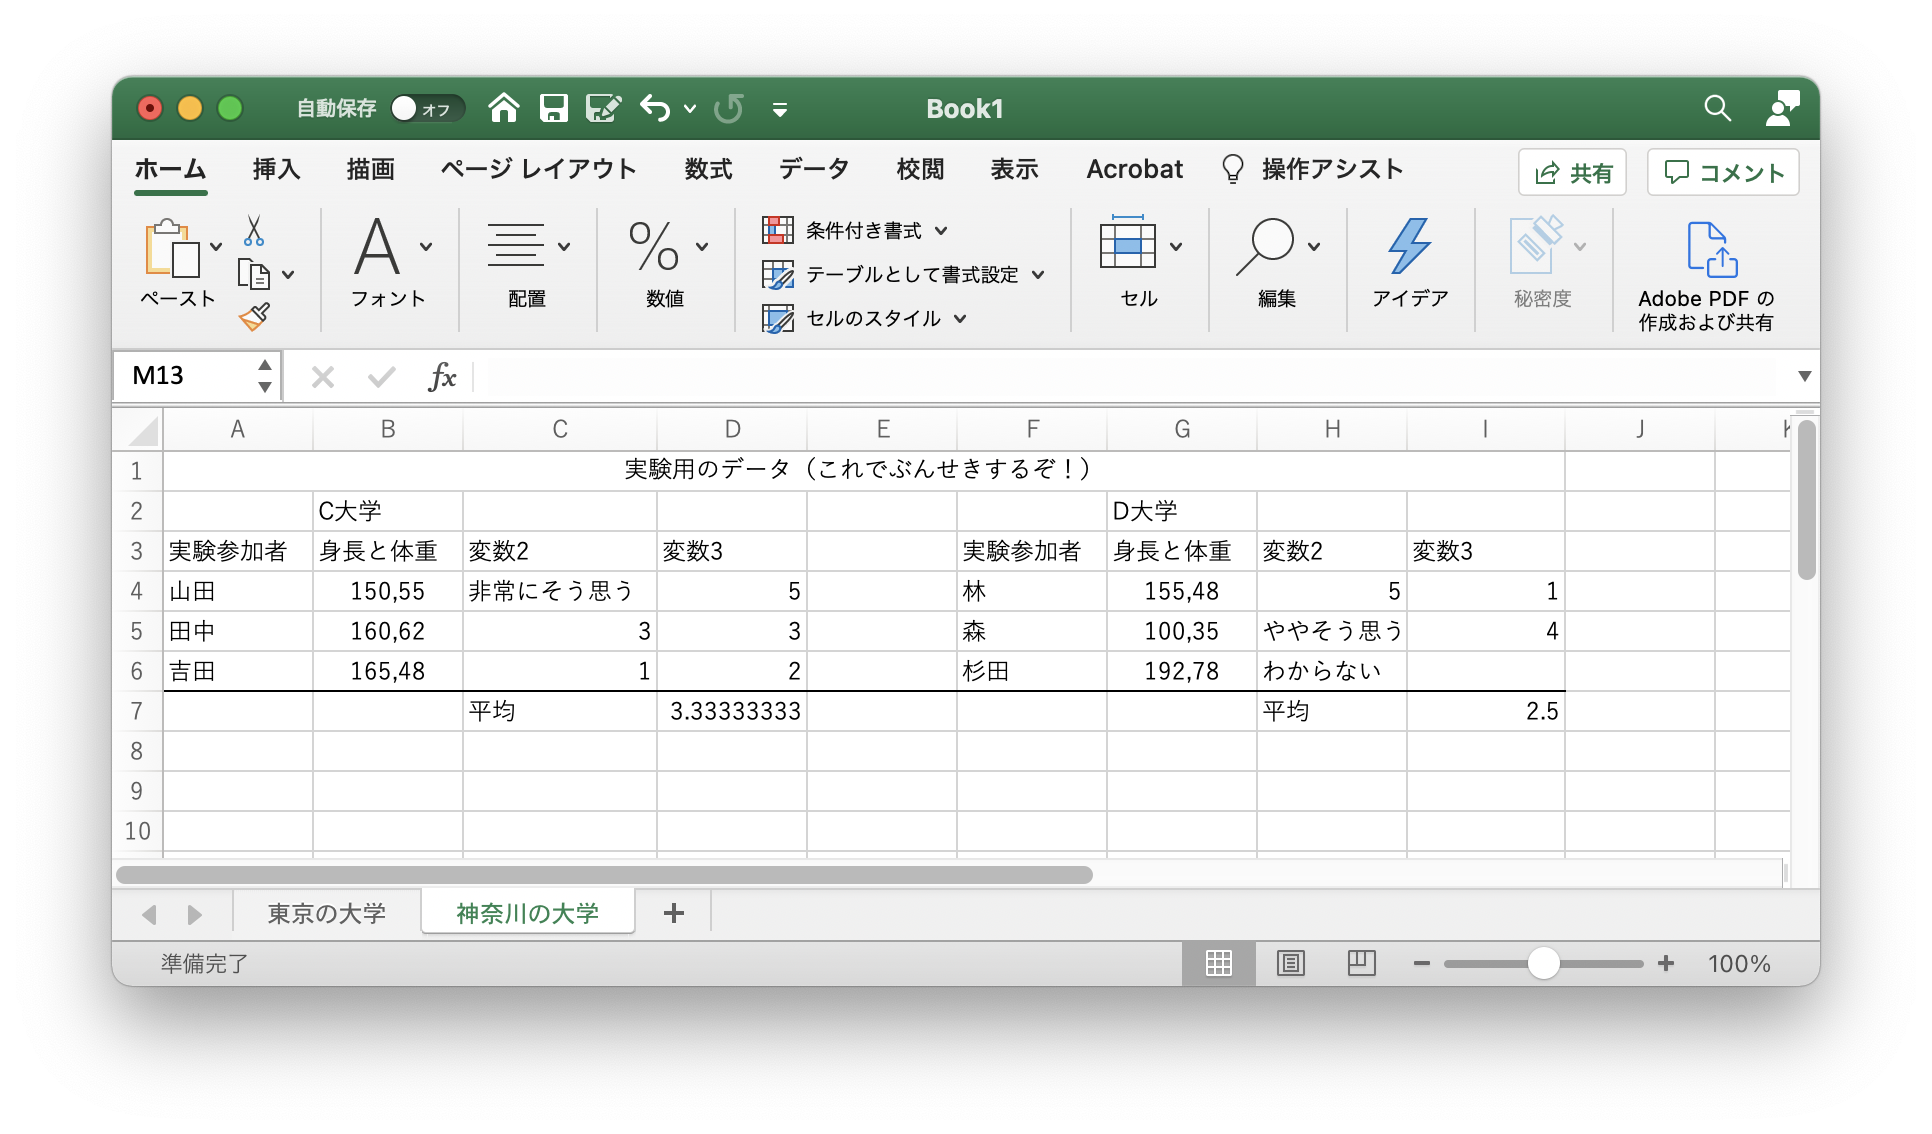
\includegraphics[keepaspectratio,width=\linewidth]{figures/20_anovakun/dataSheet.png}
\end{center}

分析しにくいよくないデータになっているのは次の箇所です。
\begin{enumerate}
	\item 1行目にこの表のタイトルのようなものが入っていますが，これは分析には使わない情報なので不要です。
	\item 1行目はセルを結合しています。データセットは\texttt{data.frame}型のように矩形であるべきなので，データのサイズを狂わせる行の存在は不適切です。
	\item 2行目には大学名が入っているようです。AからD列はC大学，FからIはD大学のデータのようですが，1つのデータセットに複数のデータが混在しているのはよくありません。
	\item 身長と体重，という変数名のところには1つのセルに複数の数字が入っています。カンマで区切られており，見た目にはわかりますが，機械的には(カンマのせいで)数字ではなく文字列として扱われます。データがデータになっていないのです。
	\item 変数2の列は「非常にそう思う」という言葉の回答と，数字が入っています。1つの列の中に複数の種類のデータが含まれるので分析できません(文字と数字の集計ができない。ちなみにこの場合は文字変数として扱われます)。
	\item 7行目に平均とありますが，データの平均はデータから計算できる量なので，Rで算出するものです。データの中に計算結果を入れておくべきではありません。
	\item I列6行目，D大学の杉田さんに関する変数3の箇所が空欄です。これはデータが入手できなかったところかもしれませんが，これは欠測値であることを明示すべきです。
	\item 「東京の大学」と「神奈川の大学」という複数のシートがあります。データファイルとしては1つのシートにすべての情報が入っていなければなりません。同時に分析できるデータなのであれば，一枚のシートにまとめるべきです。
\end{enumerate}
皆さんはいくつ気づいたでしょうか。これらの問題点を通じて言えることは「1つのデータセット，1つのセルには過不足ない情報を入れる」ということです。表を作って見せるのであればこのような入力でも良いのですが，ここでは数値データを分析することが目的なのですから，レイアウトや数字でない情報，計算してここから作れる情報は，分析に必要のない過剰な情報なのです。ちなみにアンダーラインや文字色，セルの色などは分析のときに自動的に抜け落ちます(データではない情報なので)。表計算ソフトは数字を表にして計算するソフトウェアであり，方眼用紙やレイアウトする文書とは異なることを意識しましょう。

加えて分析のときに不便なのは，文字と数字の関係です。1つのセルに複数の数字が入る場合，区切り記号などをつけることが多いかと思いますが(スペースも機械にとっては文字です！)，こうした文字種・変数の種類・水準が混在しているのも情報過多ということになります。

今回の問題点を修正したのが図\ref{fig:app_gooddata_02}のようなデータセットです。単一のデータセットで完結しています。また1つの列に一種類の変数，不要な情報はなく，過剰な情報もないデータセットになっているのがわかるかと思います。なお，変数3のところに\texttt{NA}とあるのは\texttt{No Answer}の略で\keyterm{欠測値}{けっそくち}{missing value}を意味しています。これは読み込むときに，欠測値をどのような文字にしているか，という指定ができますので問題になりません。
\begin{center}
	\captionof{figure}{分析に適したデータファイル}
	\label{fig:app_gooddata_02}
	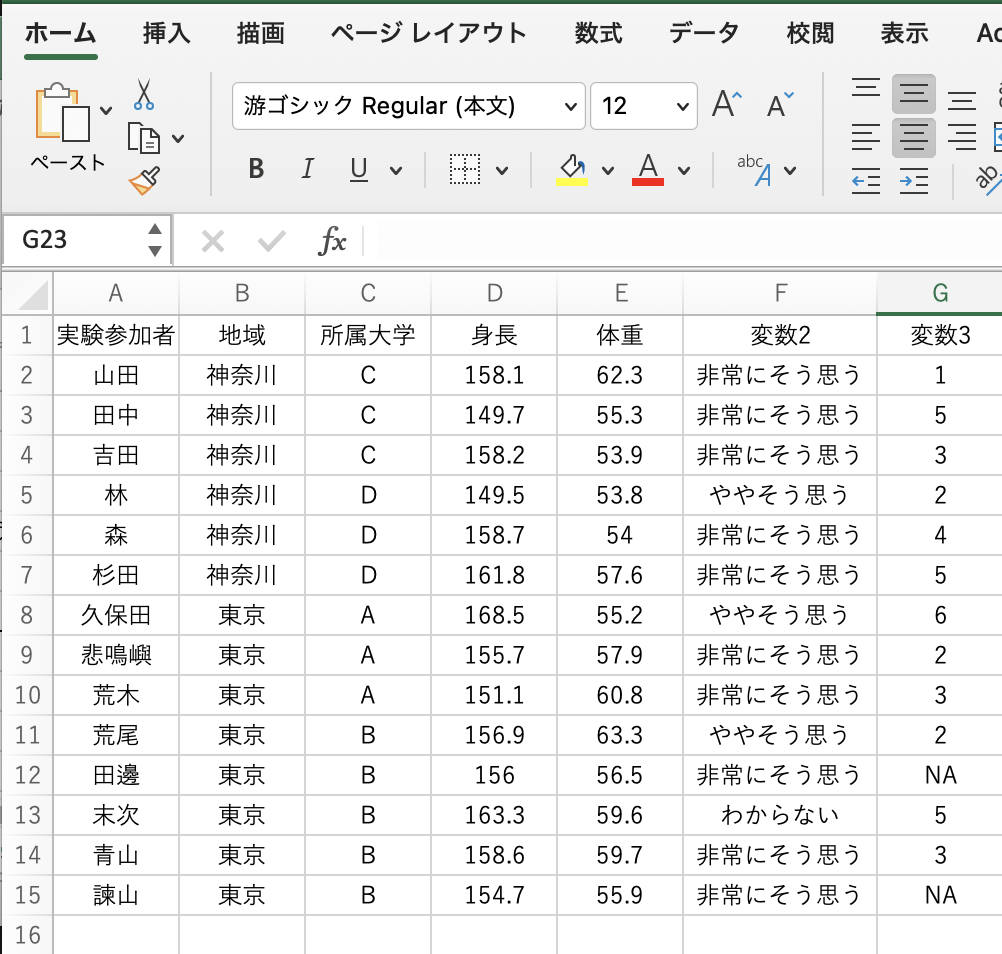
\includegraphics[keepaspectratio,width=0.8\linewidth]{figures/20_anovakun/dataSheet2.png}
\end{center}

このように，データの入力の基本は，\textbf{1行に1ケースの情報が入っている，過不足のない1つのデータセットを作ること}である，と言えます。

このようにして作られたデータファイルは，UTF-8の文字コードによるcsv形式で保存するのが基本です($\to$第\ref{computer}講，\ref{suffix}節，Pp.\pageref{suffix}参照)。ファイルを保存するときに，ファイル形式をしっかり指定し，拡張子も\texttt{.csv}にしましょう。csvファイルはASCIIファイルですし，文字コードも世界基準のUTF-8にしておけばどのPCからでもみることができます。ある一企業が開発した特定のOS，特定のアプリケーションを持っていなければデータを見ることができない，というのは科学的研究の観点からは不適切なのです。

ちなみに2020年12月，総務省により機械判読可能なデータの表記方法の統一ルールが策定されました\parencite{soumu}。それには次のようなチェック項目が含まれています。
\begin{description}
	\item[チェック項目1-1] ファイル形式はExcelかCSVとなっているか
	\item[チェック項目1-2] 1セル1データとなっているか
	\item[チェック項目1-3] 数値データは数値属性とし，文字列を含まないこと
	\item[チェック項目1-4] セルの結合をしていないか
	\item[チェック項目1-5] スペースや改行等で体裁を整えていないか
	\item[チェック項目1-6] 項目名を省略していないか
	\item[チェック項目1-7] 数式を使用している場合は，数値データに修正しているか
	\item[チェック項目1-8] オブジェクトを使用していないか
	\item[チェック項目1-9] データの単位を記載しているか
	\item[チェック項目1-10] 機種依存文字を使用していないか
	\item[チェック項目2-1] データが分断されていないか
	\item[チェック項目2-2] 1シートに複数の表が掲載されていないか
\end{description}
みなさんも自分でデータを作るときは，こうした基準に沿うように心がけてください。
また表計算ソフトの中で，代表値を計算したりグラフを書いたりしたくなりますが，みなさんは既に統計環境を手に入れているのですから，そうした加工・可視化などはRのほうでやり，データは「誰が触っても良いプレーンな素材」として保管しておくように心がけましょう。
